% thesis.tex
%
%
% Sample document to demonstrate the uwthesis document class, for theses
% in the University of Wales, Aberystwyth.
%
% You should also have received the files uwthesis.cls, mybib.bib and
% README together with this file, if not complain to the person you got
% it from.
%
% Richard Huss <rah94@aber.ac.uk>, 17 Dec 1997.
% Sorry, the README seems to have disappeared.
% Edel Sherratt, <eds@aber.ac.uk> 15 Jan 2018, 23 July 2018

\documentclass{mscthesis}
\usepackage{graphicx}
\usepackage{subfigure}

\usepackage{authordate1-4} % Use this to get Harvard/author-date style referencing

% Include the nolof and/or nolot option for no lists of figures and
% tables respectively, if required. For example,
%  \documentclass[nolof,nolot]{uwthesis}
% will produce a thesis with neither. Useful if you have no figures
% or tables.

% Load any additional LaTeX packages you need here

% Information about this thesis

\title{What I did for my MSc Project}    % Your thesis title
\author{Jon Doe}                      % Your name
\dept{Department of Computer Science} % Your department
\supervisor{Dr Who}                   % Your supervisor's name
\module{CSM9060}                      % Your module code (CSM9060, CHM9360, etc.)
\degree{MSc Data Science}             % Your degree (MSc Computer Science (Software Engineering), MSc Data Science, MSc Statistics for Computational Biology)

\begin{document}
\setlength{\parindent}{0pt}
  % Set the default line spacing. If you want double spacing the
  % default, use \doublespacing instead of \onehalfspacing.

  \onehalfspacing

  % But the preface stuff is single-spaced
  \begin{singlespace}

  % Generates the title page, signature pages etc.
  \beforepreface

  % 'Preface' type sections are introduced with \prefacesection.
  \prefacesection{ABSTRACT}

    % Replace with your abstract
    The abstract stands alone as a very short version of the dissertation.
    
    The abstract should state the scope and principal objectives of the project, describe the methods, summarize the results and state the principal conclusions.
    

  \prefacesection{ACKNOWLEDGEMENTS}

    % Replace with your acknowledgments

  %\prefacesection{\ }  % A blank section title, just to force a new page
  % Replace with your dedication

    \null\vskip1.5in
    \begin{center}

    To whoever has the patience to read this :-)
    
    This section is customary, but not obligatory.  It makes a brief statement of thanks to those who have helped.

    \end{center}

  % Insert the table of contents and lists of tables and figures
  \afterpreface

  % Double (or one-half) spacing from here onwards
  \end{singlespace}

% Your thesis goes here!
\chapter{Introduction}

Background to the project, motivation, leading to project aims and objectives.

\chapter{Literature review}

The literature review is all about the related knowledge that you are building on.  Similar products and related research are usual.

Remember to use your own words and to show relevance to your project aim.
The literature review will refer extensively to the bibliography.  Harvard (author-date) and IEEE reference styles are usual in Computer Science, but the only real rule is that you should use a consistent style.

Here is an example reference to inky matters~\cite{Jones2010}. 

Refereed articles are generally considered to have the greatest authority, but for a Computer Science project you are also likely to cite other sources, such as technical documents, user manuals, standards documents, web pages and books.

When you cite a web source, make sure to include the date of access.

\chapter{Reporting on the project -- the core chapters}

Reporting on the project will normally require more than one chapter.
A development project is likely to have chapters addressing requirements, design, implementation, testing and packaging if a plan-driven method is used.  If an agile approach is taking, you might have a chapter for each sprint or iteration.
Other kinds of project will have chapters that are appropriate to the project in question.

You are likely to include diagrams or images in your core chapters.

\begin{figure}
	\label{fig-website}
	\begin{center}
		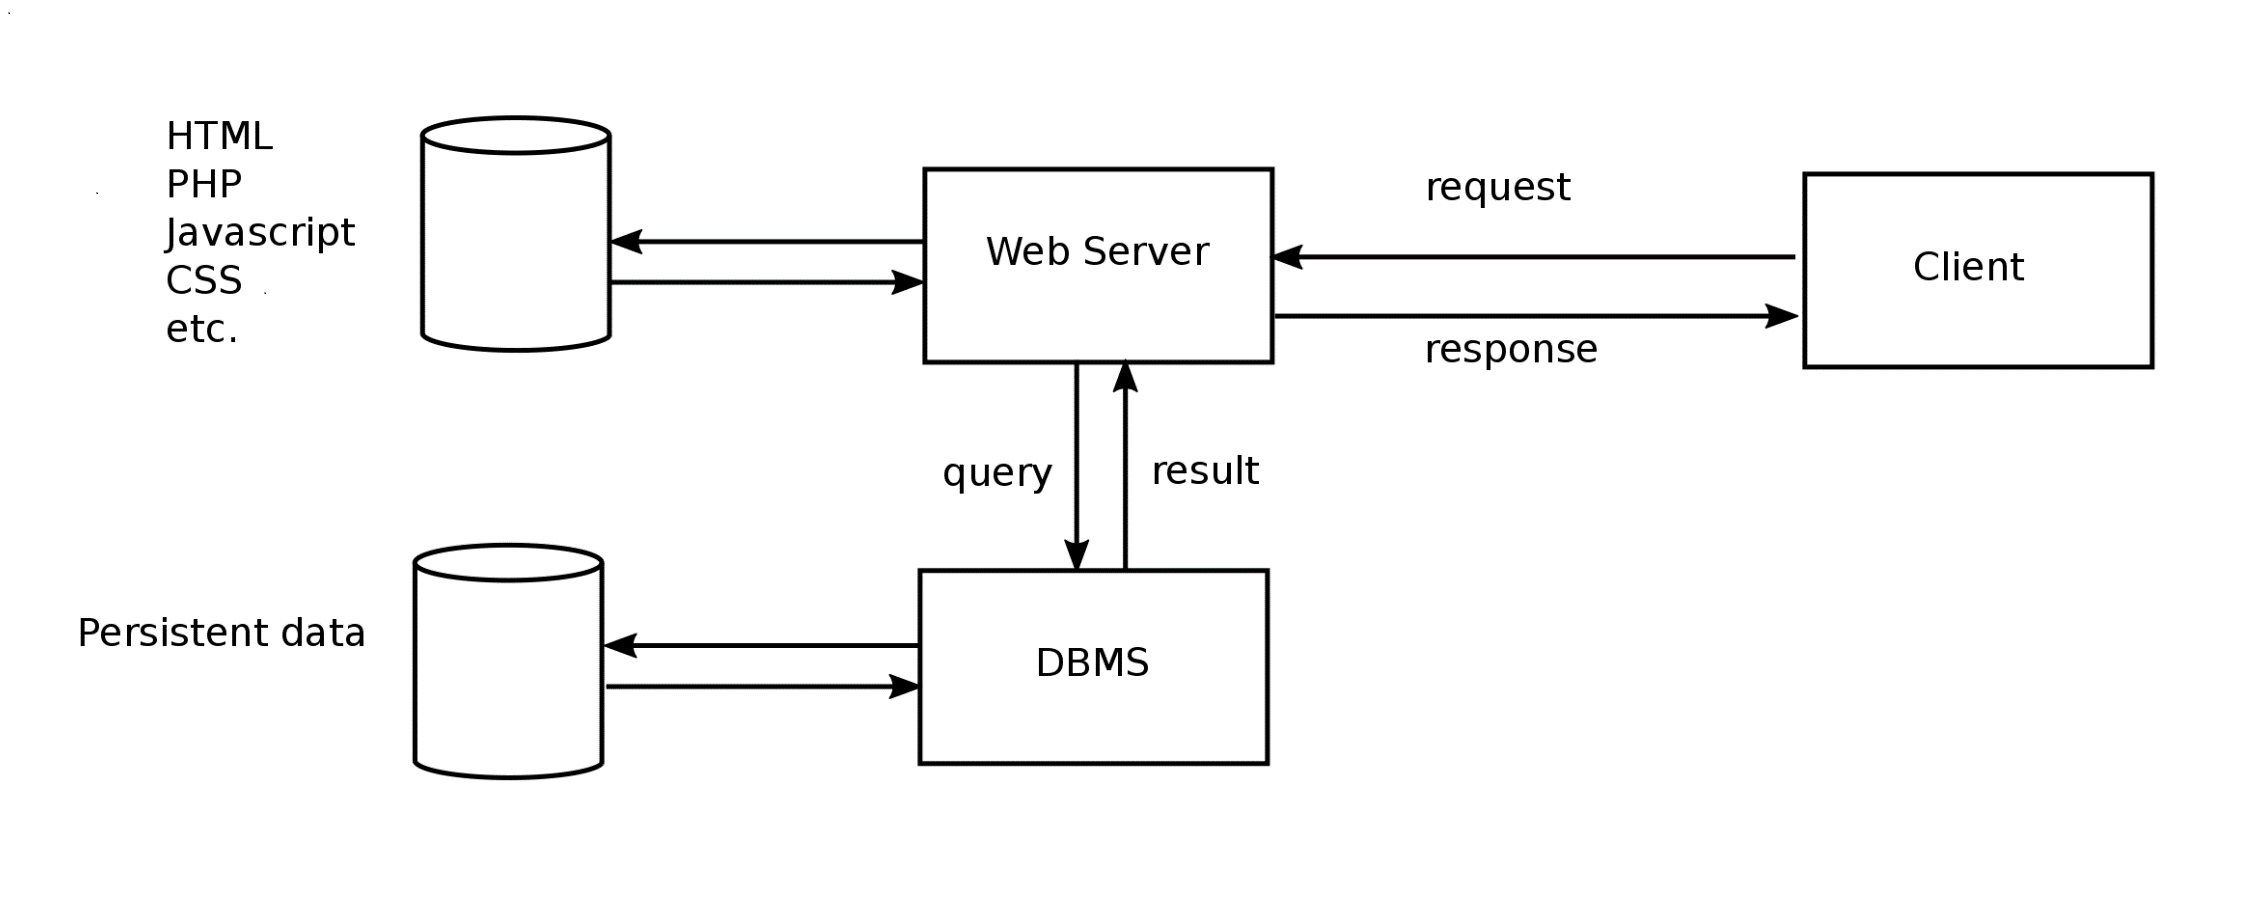
\includegraphics[width=30em]{DynamicWebsite.png}
		\caption{Structure of a dynamic website (Edel Sherratt)}
	\end{center}
\end{figure}

\chapter{Critical Evaluation}

In this chapter (it won’t be chapter 4, but probably chapter 6 or 7 once all the core chapters have been added.)

The critical evaluation consists of a discussion, leading to conclusion.  It is an essential part of a master’s degree.

It shows that you can not only carry out a substantial piece of work, but that you can reflect on it, and think critically about how you might have done it better.

Examiners view the critical evaluation as very important.

\chapter{Conclusion}

A brief summary of all that has gone before.

May include some directions for future work.


\bibliographystyle{ieee}
\bibliography{mybib}  % Pathname of your bibTeX file

\end{document}
